\documentclass[11pt, a4paper]{article}

\usepackage[english]{babel}
\usepackage{sleek}
\usepackage{common}

\title{Introduction to Artificial Intelligence (INFO8006)}
\subtitle{Exercises 3 -- Reasoning under uncertainty}
\date{\today}

\begin{document}

\maketitle

\section*{Learning outcomes}

At the end of this session you should be able to
\begin{itemize}[noitemsep]
    \item calculate marginal and conditional probabilities given joint distributions;
    \item apply and understand the Bayes rule;
    \item formulate a random process as a Bayesian network and conditional probability tables;
    \item determine whether random variables are independent given a Bayesian network;
    \item compute probabilities in the context of a (simple) Bayesian network.
\end{itemize}

\section{Beliefs}

Let $A$ and $B$ be two \emph{events} over the probability space $\Omega$. An agent holds the beliefs $P(A) = 0.4$ and $P(B) = 0.3$. What ranges of probabilities would it be rational for the agent to hold for the events $A \cup B$ and $A \cap B$ ? What if the agent also believes that $P(A | B) = 0.5$ ?

\begin{solution}
    \begin{enumerate}
        \item The agent's beliefs should satisfy
        \begin{alignat*}{2}
            0.4 = \max \cbk{P(A), P(B)} & \leq P(A \cup B) && \leq \min \cbk{1, P(A) + P(B)} = 0.7 \\
            0 = \max \cbk{0, P(A) + P(B) - 1} & \leq P(A \cap B) && \leq \min \cbk{P(A), P(B)} = 0.3 .
        \end{alignat*}
        This can be illustrated with Venn diagrams.

        \item If the agent believes that $P(A | B) = 0.5$, it should also believe that
        \begin{equation*}
            P(A \cap B) = P(A | B) P(B) = 0.5 \times 0.3 = 0.15,
        \end{equation*}
        thanks to Bayes rule. Then, the agent should rationally believe that
        \begin{equation*}
            P(A \cup B) = P(A) + P(B) - P(A \cap B) = 0.4 + 0.3 - 0.15 = 0.55.
        \end{equation*}
    \end{enumerate}
\end{solution}

\newpage

\section{(AIMA, Ex 13.8)}

\begin{table}[h]
    \centering
    \begin{tabular}{|c|c|c|c|c|}
        \hline
        & \multicolumn{2}{c|}{toothache} & \multicolumn{2}{c|}{no toothache} \\ \hline
        & catch & no catch & catch & no catch \\ \hline
        cavity & 0.108 & 0.012 & 0.072 & 0.008 \\ \hline
        no cavity & 0.016 & 0.064 & 0.144 & 0.576 \\ \hline
    \end{tabular}
\end{table}

Given the hereabove probability table, compute the following probabilities:

\begin{solution}
    In the following, we represent the events $toothache$, $catch$ and $cavity$ by the random variables $T, CT, CV: \Omega \mapsto \cbk{0, 1}$, respectively. Then, the hereabove table represents the joint probability distribution $P(T, CT, CV)$. When clear from context, we abbreviate the probability of a realization $(t, ct, cv)$ by $P(t, ct, cv)$ instead of $P(T = t, CT = ct, CV = cv)$.
\end{solution}

\begin{enumerate}
    \item $P(toothache)$

    \begin{solution}
        \begin{equation*}
            P(T = 1) = \sum_{ct} \sum_{cv} P(T = 1, ct, cv) = 0.108 + 0.012 + 0.016 + 0.064 = 0.2
        \end{equation*}
    \end{solution}

    \item $P(cavity)$

    \begin{solution}
        \begin{equation*}
            P(CV = 1) = \sum_{t} \sum_{ct} P(t, ct, CV = 1) = 0.108 + 0.012 + 0.072 + 0.008 = 0.2
        \end{equation*}
    \end{solution}

    \item $P(toothache | cavity)$

    \begin{solution}
        \begin{align*}
            P(T = 1 | CV = 1) = \frac{P(T = 1, CV = 1)}{P(CV = 1)} & = \frac{\sum_{ct} P(T = 1, ct, CV = 1)}{P(CV = 1)} \\
            & = \frac{0.108 + 0.012}{0.2} = 0.6
        \end{align*}
    \end{solution}

    \item $P(cavity | toothache \cup catch)$

    \begin{solution}
        \begin{align*}
            P(CV = 1 | T = 1 \cup CT = 1) & = \frac{P(T = 1 \cup CT = 1, CV = 1)}{P(T = 1 \cup CT = 1)} \\
            & = \frac{P(CV = 1) - P(T = 0, CT = 0, CV = 1)}{1 - P(T = 0, CT = 0)} \\
            & = \frac{0.2 - 0.008}{1 - 0.584} = \num{0.4615}
        \end{align*}
    \end{solution}

\end{enumerate}

\newpage

\section{(AIMA, Ex 13.15)}

After your yearly checkup, the doctor has bad news and good news. The bad news is that you tested positive for a serious disease and that the test is \qty{99}{\percent} accurate, \ie{} the probability of testing positive when you do have the disease is \num{0.99} and the probability of testing positive when you don't is \num{0.01}. The good news is that this is a rare disease, striking only 1 in \num{10000} people of your age. Why is it good news that the disease is rare? What are the chances that you actually have the disease?

\begin{solution}
    It is a good news because the conditional probability will drop due to the weak prior value. Indeed,
    \begin{align*}
        P(d | t) & = \frac{P(t | d) P(d)}{P(t)} \\
        & = \frac{P(t | d) P(d)}{P(t | d) P(d) + P(t | \neg d) P(\neg d)} \\
        & = \frac{0.99 \times \num{e-4}}{0.99 \times \num{e-4} + 0.01 \times (1 - \num{e-4})} = \num{0.0098} .
    \end{align*}
\end{solution}

\newpage

\section{(AIMA, Ex 13.13)}

For each of the following statements, either prove it is valid or give a counterexample.

\begin{enumerate}
    \item If $P(a | b, c) = P(b | a, c)$, then $P(a | c) = P(b | c)$.

    \begin{solution}
        True. By the conditional probability rule we have $P(a | b, c) P(b, c) = P(b | a, c) P(a, c)$, which by assumption reduces to $P(b, c) = P(a, c)$ and thereby $P(b | c) = P(a | c)$.
    \end{solution}

    \item If $P(a | b, c) = P(a)$, then $P(b | c) = P(b)$.

    \begin{solution}
        False. The statement $P(a | b, c) = P(a)$ merely states that $a$ is independent of $b$ and $c$, it makes no claim regarding the dependence of $b$ and $c$. Counterexample: $a$ and $b$ record the results of two independent coin flips, and $c = b$.
    \end{solution}

    \item If $P(a | b) = P(a)$, then $P(a | b, c) = P(a | c)$.

    \begin{solution}
        False. While the statement $P(a | b) = P(a)$ implies that $a$ is independent of $b$, it does not imply that $a$ is conditionally independent of $b$ given $c$. Counterexample: $a$ and $b$ record the results of two independent coin flips, and $c = a \vee b$.
    \end{solution}
\end{enumerate}

\newpage

\section{Bag of coins}

We have a bag of three biased coins $a$, $b$, and $c$ with probabilities of coming up heads of \qty{20}{\percent}, \qty{60}{\percent}, and \qty{80}{\percent}, respectively. One coin is drawn randomly from the bag (with equal probability of drawing each of the three coins), and then the coin is flipped three times to generate the outcomes $X_1$, $X_2$ and $X_3$ (heads or tail).

\begin{enumerate}
    \item Draw the Bayesian network corresponding to this setup and define the corresponding conditional probability tables (CPTs).

    \begin{solution}
        The process is described with the following random variables:
        \begin{itemize}
            \item $Y \in \cbk{a, b, c}$, the coin drawn from the bag.
            \item $X_i \in \cbk{h, t}$, the realization of the $i$-th coin toss.
        \end{itemize}
        The variable $Y$ is the parent of $X_i$, it should be put before in the network ordering.

        \begin{figure}[h]
            \begin{subfigure}[c]{0.495\textwidth}
                \centering
                \begin{tikzpicture}[node distance = 2cm]
                    \node[state] (Y) {$Y$};
                    \node[state] (X1) [below left of=Y] {$X_1$};
                    \node[state] (X2) [below of=Y] {$X_2$};
                    \node[state] (X3) [below right of=Y] {$X_3$};

                    \draw[arrow] (Y) to (X1);
                    \draw[arrow] (Y) to (X2);
                    \draw[arrow] (Y) to (X3);
                \end{tikzpicture}
            \end{subfigure}
            \begin{subfigure}[c]{0.495\textwidth}
                \centering
                \begin{tabular}{c|cc}
                    \toprule
                     $Y$ & $P(Y)$ & $P(X_i = h | Y)$ \\
                     \midrule
                     $a$ & $\frac{1}{3}$ & $0.2$ \\
                     $b$ & $\frac{1}{3}$ & $0.6$ \\
                     $c$ & $\frac{1}{3}$ & $0.8$ \\
                    \bottomrule
                \end{tabular}
            \end{subfigure}
        \end{figure}
    \end{solution}

    \item Determine which coin ($a$, $b$ or $c$) is most likely to have been drawn from the bag if the observed tosses came out heads twice and tail once.

    \begin{solution}
        In order to find the most likely coin, we have to calculate the conditional probability distribution $P(Y | X_1 = h, X_2 = h, X_3 = t)$\footnote{It should be noted that the order of the tosses is irrelevant as they are performed independently.}. Thanks to Bayes rule, we have
        \begin{equation*}
        P(Y | X_1 = h, X_2 = h, X_3 = t) = \alpha P(X_1 = h, X_2 = h, X_3 = t | Y) P(Y).
        \end{equation*}
        But we know that $X_1$, $X_2$ and $X_3$ are independent with respect to $Y$, meaning that
        \begin{equation*}
            P(X_1, X_2, X_3 | Y) = P(X_1 | Y) P(X_2 | Y) P(X_3 | Y).
        \end{equation*}
        Then, we have
        \begin{equation*}
            P(Y | X_1 = h, X_2 = h, X_3 = t) = \alpha \times \frac{1}{3} \times \begin{cases}
                0.2 \times 0.2 \times 0.8 = \num{0.032} & \text{if } Y = a \\
                0.6 \times 0.6 \times 0.4 = \num{0.144} & \text{if } Y = b \\
                0.8 \times 0.8 \times 0.2 = \num{0.128} & \text{if } Y = c \\
            \end{cases}
        \end{equation*}
        meaning that $b$ is the most likely coin to have been drawn. Interestingly, we don't need to normalize the distribution as we only care about the maximum.
    \end{solution}
\end{enumerate}

\newpage

\section{Handedness (AIMA, Ex 14.6)}

Let $H_x$ be a random variable denoting the handedness of an individual $x$, with possible values $l$ or $r$. A common \emph{hypothesis} is that left or right-handedness is inherited by a simple mechanism; that is, there is a gene $G_x$, also with values $l$ or $r$, and $H_x$ turns out the same as $G_x$ with some probability $s$.

Furthermore, the gene itself is equally likely to be inherited from either of the individual's parents, with a small nonzero probability $m$ of a random mutation flipping the gene.

\begin{enumerate}
    \item Which of the following networks claim that $P(G_{child} | G_{mother}, G_{father}) = P(G_{child})$ ?

    \begin{figure}[h]
        \centering
        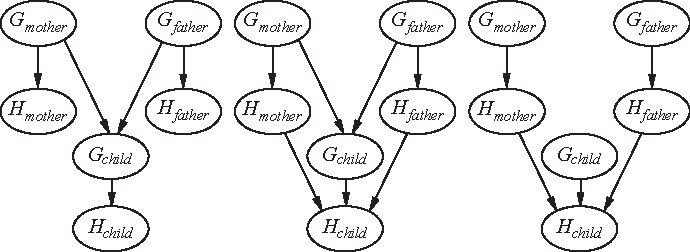
\includegraphics[width=0.9\textwidth]{figures/e3_handedness.pdf}
    \end{figure}

    \begin{solution}
        The third one, as the node $G_{child}$ does not have any parents.
    \end{solution}

    \item Which of the networks make independence claims that are consistent with the hypothesis about the inheritance of handedness ?

    \begin{solution}
        The first and second ones. It should be noted that the second one is also valid as it makes \emph{less} assumptions about the variables dependencies, \ie{} it is more general than the first one.
    \end{solution}

    \item Write down the CPT for the $G_{child}$ nodes in first network, in terms of $s$ and $m$.

    \begin{solution}
        \begin{table}[h]
            \centering
            \begin{tabular}{cc|c}
                \toprule
                 $G_{mother}$ & $G_{father}$ & $P(G_{child} = l | G_{mother}, G_{father})$ \\
                 \midrule
                 $l$ & $l$ & $1 - m$ \\
                 $l$ & $r$ & $0.5$ \\
                 $r$ & $l$ & $0.5$ \\
                 $r$ & $r$ & $m$ \\
                \bottomrule
            \end{tabular}
        \end{table}
    \end{solution}

    \item Suppose that $P(G_{mother} = l) = P(G_{father} = l) = q$. In the first network, derive an expression for $P(G_{child} = l)$ in terms of $s$, $m$ and $q$.
    \begin{solution}
        \begin{align*}
            P(G_{child} = l) & = \sum_{g_m} \sum_{g_f} P(G_{child} = l, g_m, g_f) \\
            & = \sum_{g_m} \sum_{g_f} P(G_{child} = l | g_m, g_f) P(g_m) P(g_f) \\
            & = (1 - m) q^2 + 0.5 (1 - q) q + 0.5 q (1 - q) + m (1 - q)^2 \\
            & = q + m - 2qm
        \end{align*}
    \end{solution}

    \item Under conditions of genetic equilibrium, we expect the distribution of genes to be the same across generations. Use this to calculate the value of $q$, and, given what you know about handedness in humans, explain why the hypothesis described at the beginning of this question must be wrong.

    \begin{solution}
        Under genetic equilibrium, we have $P(G_{child} = l) = P(G_{parent} = l) = q$. Therefore, $q = q + m - 2 q m$ meaning that $q = 0.5$. In practice, being left-handed is much more rare than being right-handed which invalidates the initial hypothesis.
    \end{solution}
\end{enumerate}

\newpage

\section{Independence}

\begin{figure}[h]
    \centering
    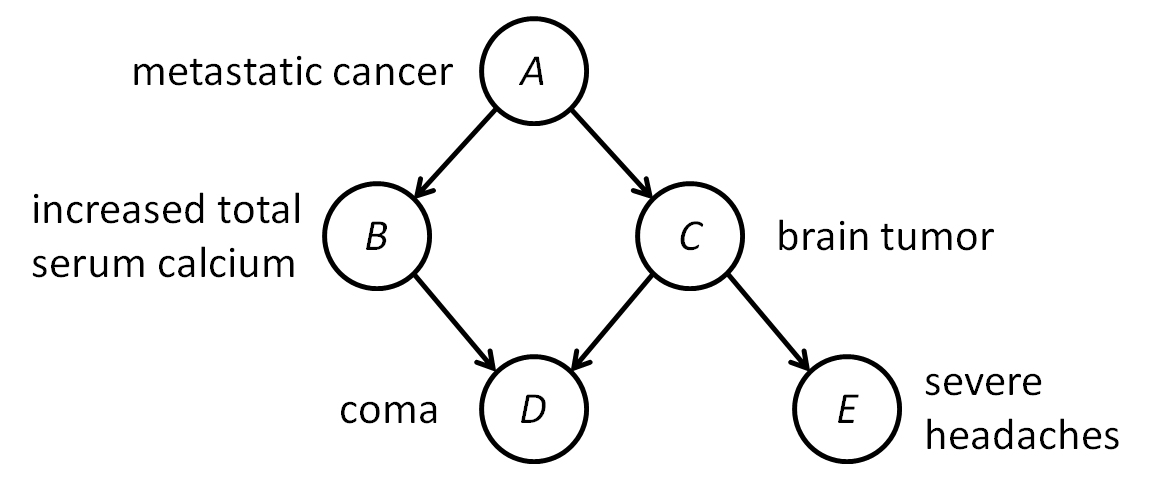
\includegraphics[width=0.6\textwidth]{figures/e3_independence.png}
\end{figure}

Considering the hereabove Bayesian network, which of the following statements are enforced by the network structure?

\begin{solution}
    We apply the d-separation\footnote{Slides 64 and 65, Lecture 4.} algorithm. To show that two variables $X$ and $Y$ could be dependent, it is sufficient to find a single \emph{active} (undirected) path from $X$ to $Y$. A path is active if all of its consecutive triples are active.
\end{solution}

\begin{enumerate}
    \item $P(B, C) = P(B) P(C)$

    \begin{solution}
        This is true iff (if and only if) $B \perp C$ ($B$ is independent from $C$). The two paths that link $B$ and $C$ are $(B, A, C)$ and $(B, D, C)$. $(B, A, C)$ is active because $A$ is unknown ($\wedge$-structure). We cannot guarantee that $B \perp C$.
    \end{solution}

    \item $P(B, C | A) = P(B | A) P(C | A)$

    \begin{solution}
        This is true iff $B \perp C | A$. This time, $(B, A, C)$ is not active because $A$ is known. $(B, D, C)$ is not active either because $D$ is unknown ($\vee$-structure). We can guarantee that $B \perp C | A$.
    \end{solution}

    \item $P(B, C | A, D) =  P(B | A, D) P(C | A, D)$

    \begin{solution}
        This is true iff $B \perp C | A, D$. This time, $(B, D, C)$ is active because $D$ is known. We cannot assert that $B \perp C | A, D$.
    \end{solution}

    \item $P(B, E | A) = P(B | A) P(E | A)$

    \begin{solution}
        This is true iff $B \perp E | A$. We know that, knowing $A$, no path between $B$ and $C$ are active. As $C$ is the only parent of $E$, all paths between $B$ and $E$ go trough $C$, meaning that they are not active. We can guarantee that $B \perp E | A$.
    \end{solution}

    \item $P(C | A, D, E) = P(C | A, B, D, E)$

    \begin{solution}
        This is true iff $B \perp C | A, D, E$. Once again, $(B, D, C)$ is active because $D$ is known. We can cannot guarantee that $B \perp C | A, D, E$.
    \end{solution}

    \item $P(B, E) = \sum_{a, c, d} P(E | c) P(d | B, c) P(c | a) P(B | a) P(a)$

    \begin{solution}
        Since $$P(B, E) = \sum_{a, c, d} P(a, B, c, d, E),$$ we need to assess whether $$P(A, B, C, D, E) = P(E | C) P(D | B, C) P(C | A) P(B | A) P(A),$$
        is guaranteed. This factorization corresponds exactly to
        \begin{equation*}
            P(X_1, \dots, X_n) = \prod_{i = 1}^n P(X_i | parents(X_i)) ,
        \end{equation*}
        for the considered network, which we know is guaranteed.
    \end{solution}
\end{enumerate}

For the same network, use inference by variable elimination to compute $P(E | A = 1, B = 1)$.

\begin{solution}
    We have
    \begin{align*}
        P(E | A = 1, B = 1) & = \alpha \sum_{c, d} P(A = 1, B = 1, c, d, E)\\
        & = \alpha \sum_{c, d} P(A = 1) P(B = 1| A = 1) P(c| A = 1) P(d|B = 1, c) P(E|c) \\
        & = \alpha P(A = 1) P(B = 1 | A = 1) \sum_{c} P(c|A = 1) P(E|c)\sum_d P(d|B = 1,c) .
    \end{align*}
    We define the initial factors as
    \begin{align*}
        f_1 & = P(A=1) \\
        f_2 & = P(B=1 | A=1) \\
        f_3(C) & = P(C|A=1) \\
        f_4(E, C) & = P(E|C) \\
        f_5(C, D) & = P(D|B=1, C)
    \end{align*}
    and the composite factors as
    \begin{align*}
        f_6(C) & = \sum_d f_5(C, d) \\
        f_7(C, E) & = f_3(C) \times f_4(E, C) \times f_6(C) \\
        f_8(E) & = \sum_c f_7(c, E) \\
        f_9(E) & = f_1 \times f_2 \times f_7(E) .
    \end{align*}
    Finally,
    \begin{equation*}
        P(E | A = 1, B = 1) = \alpha f_9(E) = \frac{f_9(E)}{\sum_e f_9(e)}.
    \end{equation*}
\end{solution}

\newpage

\section{Car Diagnosis (AIMA, Ex 14.8)}

Let be the following Bayesian network describing some features of a car's electrical system and engine. Each variable is Boolean, and the true value indicates that the corresponding aspect of the vehicle is in working order.

\begin{figure}[h]
    \centering
    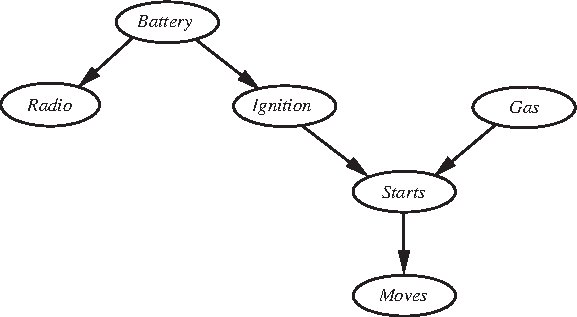
\includegraphics[width=0.6\textwidth]{figures/e3_car.pdf}
\end{figure}

\begin{enumerate}
    \item Extend the network with the Boolean variables IcyWeather and StarterMotor.

    \begin{solution}
        IcyWeather is not caused by any of the car-related variables, so needs no parents. It directly affects the battery and the starter motor. StarterMotor is an additional precondition for Starts.

        \begin{figure}[h]
            \centering
            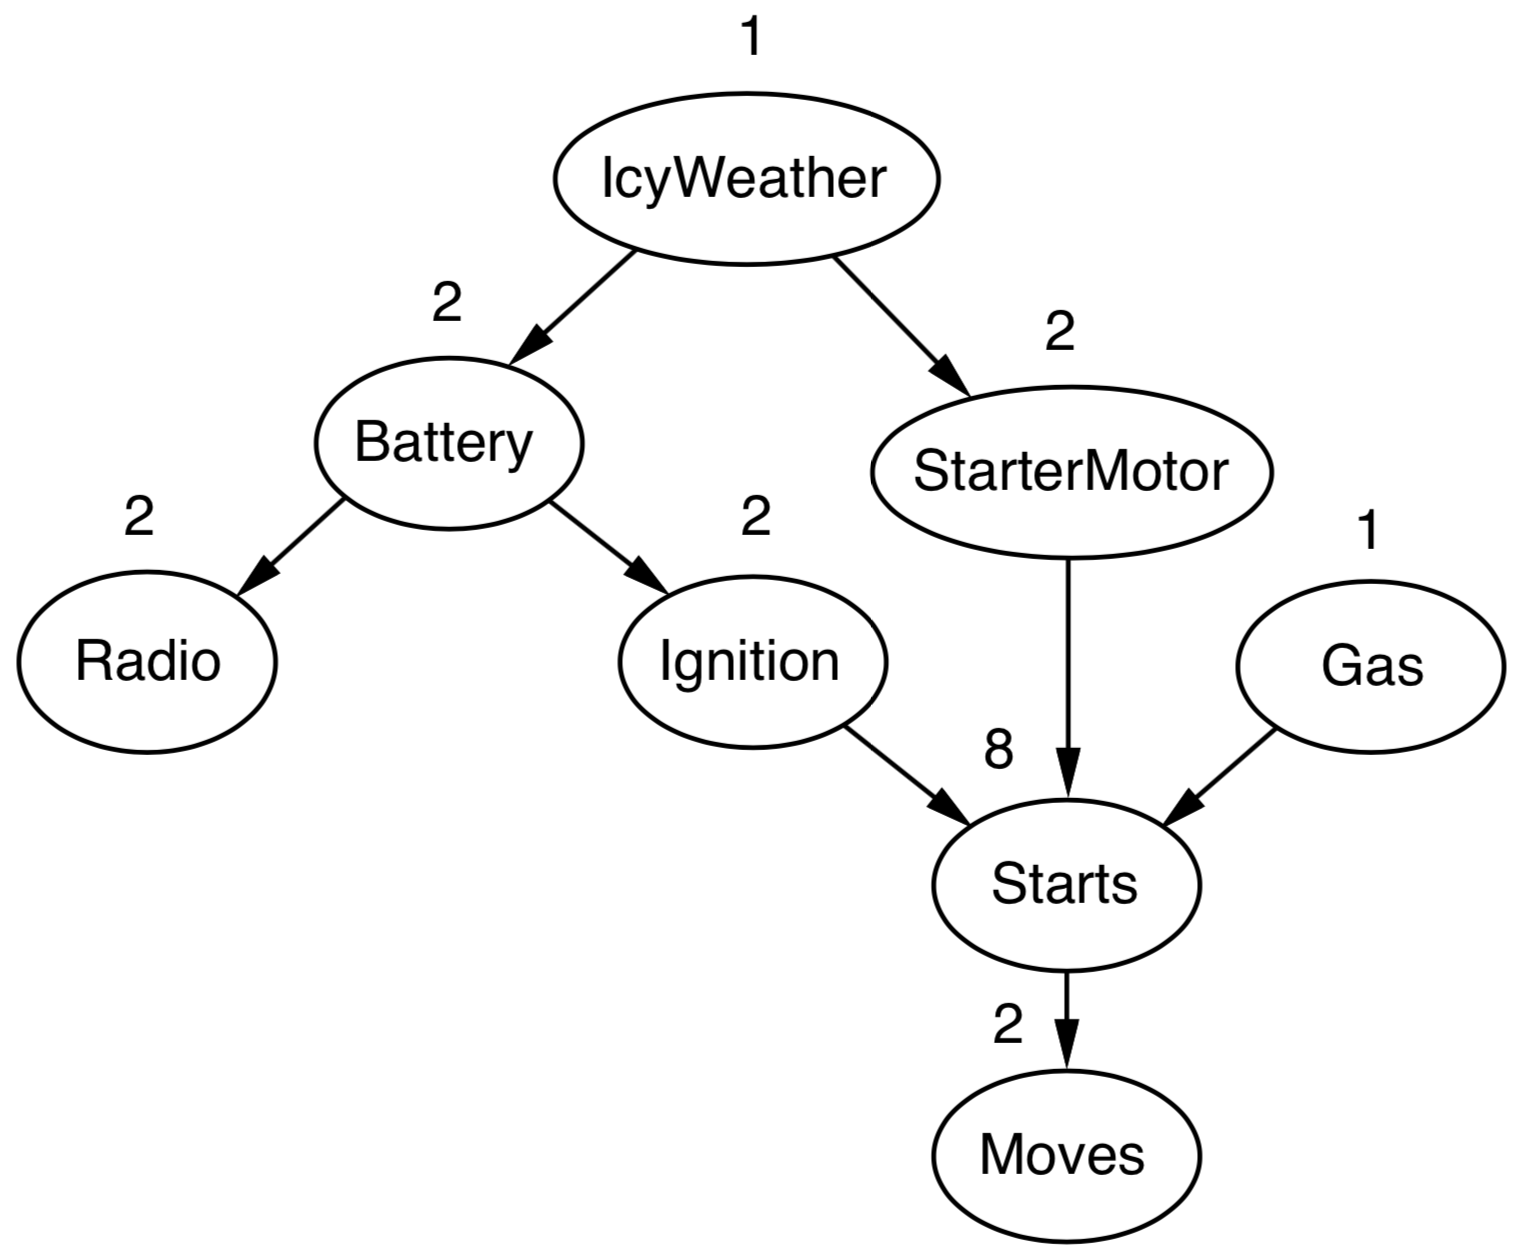
\includegraphics[width=0.6\textwidth]{figures/e3_car_full.png}
        \end{figure}
    \end{solution}

    \item According to your knowledge of cars, give reasonable conditional probability tables for all the nodes.

    \begin{solution}
        Reasonable probabilities may vary a lot depending on the kind of car and perhaps the personal experience of the assessor. The following values indicate the general order of magnitude and relative values that would be reasonable:
        \begin{itemize}
            \item A reasonable prior for IcyWeather might be $0.05$ (depending on location and season).
            \item $P(Battery|IcyWeather)=0.95,P(Battery|\lnot IcyWeather)=0.997$.
            \item $P(StarterMotor|IcyWeather) = 0.98$, $P(Battery|\lnot IcyWeather) = 0.999$.
            \item $P(Radio|Battery) = 0.9999, P (Radio|\lnot Battery) = 0.05$.
            \item $P(Ignition|Battery) = 0.998, P (Ignition|\lnot Battery) = 0.01$.
            \item $P(Gas) = 0.995$.
            \item $P(Starts|Ignition,StarterMotor,Gas) = 0.9999$, other entries $0.0$.
            \item $P(Moves|Starts) = 0.998$.
        \end{itemize}
    \end{solution}

    \item How many independent values are contained in the joint probability distribution for eight Boolean nodes, assuming that no conditional independence relations are known to hold among them?

    \begin{solution}
        With 8 Boolean variables, the joint has $2^8 - 1 = 255$ independent entries.
    \end{solution}

    \item How many independent probability values do your network tables contain?

    \begin{solution}
        Given the topology with IcyWeather and StarterMotor, the total number of independent CPT entries is $1 + 2 + 2 + 2 + 2 + 1 + 8 + 2 = 20$.
    \end{solution}
\end{enumerate}

\newpage

\section{Nuclear Power Plant (AIMA, Ex 14.11)}

In your local nuclear power station, there is an alarm that senses when a temperature gauge exceeds a given threshold. The gauge measures the temperature of the core. Consider the Boolean variables $A$ (alarm sounds), $F_A$ (alarm is faulty), and $F_G$ (gauge is faulty) and the multi-valued nodes $G$ (gauge reading) and $T$ (actual core temperature).

\begin{enumerate}
    \item Draw a Bayesian network for this domain, given that the gauge is more likely to fail when the core temperature gets too high.

    \begin{solution}
        \begin{figure}[h]
            \centering
            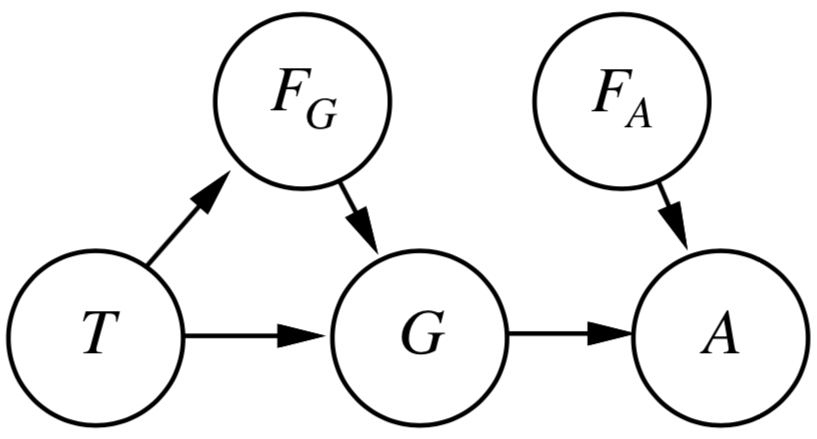
\includegraphics[width=0.4\textwidth]{figures/e3_nuclear.png}
        \end{figure}
    \end{solution}

    \item Suppose there are just two possible actual and measured temperatures: low ($l$) and high ($h$). The probability that the gauge gives the correct temperature is $x$ when it is working, but $y$ when it is faulty. Give the conditional probability table associated with $G$.

    \begin{solution}
        The CPT for $G$ is shown below. Students should pay careful attention to the semantics of $F_G$, which is true when the gauge is faulty, \ie{} not working properly.
        \begin{table}[h]
            \centering
            \begin{tabular}{cc|c}
                \toprule
                 $T$ & $F_G$ & $P(G = l | T, F_G)$ \\
                 \midrule
                 $l$ & 0 & $x$ \\
                 $l$ & 1 & $y$ \\
                 $h$ & 0 & $1 - x$ \\
                 $h$ & 1 & $1 - y$ \\
                 \bottomrule
            \end{tabular}
        \end{table}
    \end{solution}

    \item Suppose the alarm is always triggered by high measured temperatures, unless it is faulty, in which case it never sounds. Give the conditional probability table associated with $A$.

    \begin{solution}
        \begin{table}[h]
            \centering
            \begin{tabular}{cc|c}
                \toprule
                 $G$ & $F_A$ & $P(A = 1 | G, F_A)$ \\
                 \midrule
                 $l$ & 0 & 0 \\
                 $l$ & 1 & 0 \\
                 $h$ & 0 & 0 \\
                 $h$ & 1 & 1 \\
                 \bottomrule
            \end{tabular}
        \end{table}
    \end{solution}

    \item Suppose the gauge is not faulty and the alarm is triggered. Calculate an expression for the probability that the temperature of the core is too high, in terms of the various conditional probabilities in the network.

    \begin{solution}
        The probability of interest here is $P(T = h | A = 1, F_G = 0)$. Because the alarm's behavior is deterministic, we can deduce that $G$ indicates high ($h$). Hence, $P(T = h | A = 1, F_G = 0) = P(T = h | A = 1, G = h, F_G = 0)$. We also see that $A \perp T | G$. Therefore, we only need to calculate
        \begin{align*}
            P(T = h | G = h, F_G = 0) & = \frac{P(T = h, G = h, F_G = 0)}{P(G = h, F_G = 0)} \\
            & = \frac{P(G = h | T = h, F_G = 0) P(F_G = 0 | T = h) P(T = h)}{\sum_t P(G = h | t, F_G = 0) P(F_G = 0 | t) P(t)} ,
        \end{align*}
        which we cannot develop more as we don't know $P(T)$ and $P(F_G | T)$.
    \end{solution}
\end{enumerate}

\newpage

\section*{Supplementary materials}

\begin{itemize}
    \item Hygiène Mentale -- La Pensée Bayésienne

    \qrcode{https://www.youtube.com/watch?v=x-2uVNze56s}

    \item The Book of Why

    \qrcode{http://bayes.cs.ucla.edu/WHY/why-intro.pdf}

    \item Chapters 13 and 14 of the reference textbook.
\end{itemize}

\end{document}
